\documentclass[11pt,a4paper]{article}
% Share the established exercise-session typography and palette.
\usepackage[margin=18mm,headheight=24pt]{geometry}
\usepackage[T1]{fontenc}
\usepackage[english]{babel}
\usepackage{lmodern}
\usepackage{microtype}
\usepackage{amsmath,amssymb}
\usepackage{siunitx}
\usepackage{tikz}
\usetikzlibrary{arrows.meta,calc,angles,quotes}
\usepackage{enumitem}
\usepackage{xcolor}
\usepackage{fancyhdr}
\usepackage{lastpage}
\usepackage[hidelinks]{hyperref}

\definecolor{VectorGreen}{HTML}{174A38}
\definecolor{VectorAccent}{HTML}{216343}
\definecolor{VectorMint}{HTML}{E2F0E5}
\definecolor{VectorCoral}{HTML}{C45136}
\definecolor{VectorInk}{HTML}{203B31}
\definecolor{VectorMuted}{HTML}{5F7468}

\color{VectorInk}
\setlength{\parindent}{0pt}
\setlength{\parskip}{0.55em}
\setlist[enumerate]{leftmargin=*,itemsep=0.45em,topsep=0.35em}
\sisetup{per-mode=symbol}

\pagestyle{fancy}
\fancyhf{}
\lhead{\textcolor{VectorMuted}{Vectors · Exercise session}}
\rhead{\textcolor{VectorMuted}{Addition and subtraction}}
\cfoot{\textcolor{VectorMuted}{\thepage\ / \pageref*{LastPage}}}
\renewcommand{\headrulewidth}{0.4pt}
\renewcommand{\headrule}{\hbox to\headwidth{\color{VectorMint}\leaders\hrule height \headrulewidth\hfill}}

\newcommand{\sessiontitle}[2]{%
  {\color{VectorGreen}\fontsize{25}{29}\selectfont\bfseries #1\par}
  \vspace{0.2em}
  {\color{VectorMuted}\large #2\par}
  \vspace{0.55em}
  {\color{VectorAccent}\rule{\textwidth}{1.5pt}}
}

\newcommand{\problemheading}[2]{%
  {\color{VectorAccent}\small\bfseries\MakeUppercase{Problem #1}}\par
  {\color{VectorGreen}\LARGE\bfseries #2}\par
  \vspace{0.25em}
}

\newcommand{\prediction}[1]{%
  \begin{center}
  \colorbox{VectorMint}{\parbox{0.92\linewidth}{\textbf{Predict before calculating.} #1}}
  \end{center}
}

\newcommand{\checkpoint}[1]{%
  \begin{center}
  \fcolorbox{VectorAccent}{white}{\parbox{0.91\linewidth}{\textbf{Reasoning checkpoint.} #1}}
  \end{center}
}

\newcommand{\worklines}[1]{%
  \par\vspace{0.25em}
  {\color{VectorMuted}\small\textit{Working and explanation}}\par
  \foreach \n in {1,...,#1}{\vspace{0.54cm}\noindent\textcolor{VectorMint}{\rule{\linewidth}{0.35pt}}\par}
}

\newcommand{\answerbox}[1]{%
  \begin{center}
  \colorbox{VectorMint}{\parbox{0.92\linewidth}{\textbf{Answer.} #1}}
  \end{center}
}

\lhead{\textcolor{VectorMuted}{Dynamics · Exercise session 3}}
\rhead{\textcolor{VectorMuted}{Dot products · No coordinates}}


\begin{document}
\sessiontitle{Let the dot product do the seeing}{Exercise session 3 · Motion without coordinates}

Solve using vector equations and dot products, without choosing coordinate
axes or resolving vectors into components. Problems 1 and 2 are required;
Problem 3 is an optional modeling challenge.

\problemheading{1}{A familiar flight, a different route}

A projectile is launched with speed $u$ at an angle $\alpha$ above the
horizontal, where $0<\alpha<90^\circ$. Take the launch point $O$ as the
origin, and let $\vec r(t)$ be the projectile's position vector.
Gravity is uniform, with acceleration $\vec g$ of magnitude $g$.
Ignore air resistance. The projectile lands at the same height from
which it was launched.

\begin{center} 
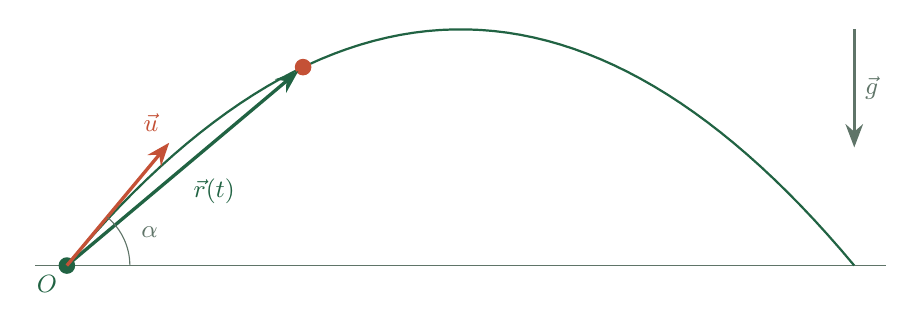
\begin{tikzpicture}[>=Stealth,font=\small]
  \draw[VectorMuted] (-0.4,0)--(10.4,0);
  \draw[thick,VectorAccent,domain=0:10,samples=60]
    plot (\x,{0.12*\x*(10-\x)});
  \fill[VectorAccent] (0,0) circle (3pt) node[below left] {$O$};
  \fill[VectorCoral] (3,2.52) circle (3pt);
  \draw[->,very thick,VectorAccent] (0,0)--(2.94,2.47)
    node[midway,below right] {$\vec r(t)$};
  \draw[->,very thick,VectorCoral] (0,0)--(1.3,1.56)
    node[above left] {$\vec u$};
  \draw[VectorMuted] (0.8,0) arc (0:50.2:0.8);
  \node[VectorMuted] at (1.05,0.42) {$\alpha$};
  \draw[->,very thick,VectorMuted] (10,3)--(10,1.5)
    node[midway,right] {$\vec g$};
\end{tikzpicture}
\end{center}

\textbf{Using only $\vec r(t)\cdot\vec r(t)$ and its derivative with
respect to time}, determine:
\begin{enumerate}[label=\alph*)]
  \item the maximum height above the launch point;
  \item the total time of flight.
\end{enumerate}

\textbf{Optional reflection.} At the highest point, is
$\vec r\cdot\vec r$ stationary? Explain physically.

\worklines{6}

\clearpage
\problemheading{2}{Three speeds, an unseen force}

A \SI{2}{kg} puck moves on a horizontal frictionless table under a constant
horizontal net force $\vec F$. A sensor records only its \textbf{speed},
not its velocity direction or position. These are its readings:

\begin{center}
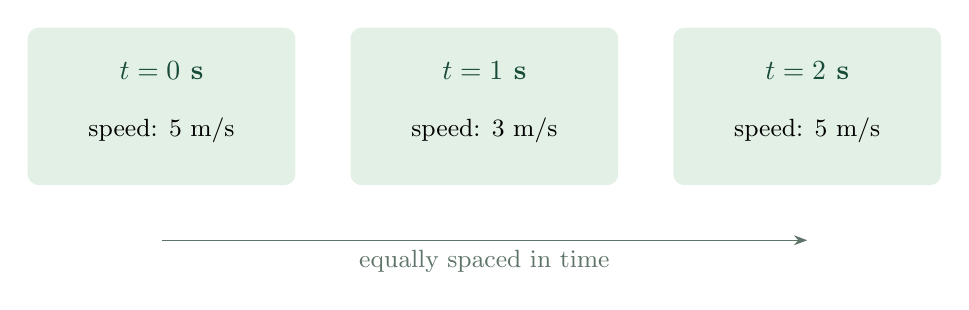
\begin{tikzpicture}[>=Stealth,font=\small]
  \foreach \x/\time in {0/0,4.1/1,8.2/2}{
    \fill[VectorMint,rounded corners] (\x,0) rectangle +(3.4,2.0);
    \node[VectorGreen,font=\bfseries] at (\x+1.7,1.45) {$t=\time$ s};
  }
  \node at (1.7,0.7) {speed: 5 m/s};
  \node at (5.8,0.7) {speed: 3 m/s};
  \node at (9.9,0.7) {speed: 5 m/s};
  \draw[->,VectorMuted] (1.7,-0.7)--(9.9,-0.7);
  \node[below,VectorMuted] at (5.8,-0.7) {equally spaced in time};
\end{tikzpicture}
\end{center}

\begin{enumerate}[label=\alph*)]
  \item Find the magnitude of $\vec F$ and the angle it makes with the
    initial velocity. Can speed readings determine the force's absolute
    direction across the table?
  \item At what time between the first and last readings is the puck
    slowest? Find that speed. Does it ever stop during this interval?
  \item Find the straight-line distance between its positions at $t=0$
    and $t=2$ s. What angle does this displacement make with $\vec F$?
\end{enumerate}

\worklines{7}

\clearpage
\problemheading{3}{What force turned it back?}
{\color{VectorCoral}\bfseries Optional · Modeling challenge}

A particle of mass $m$ approaches a fixed source $O$ along a straight line.
The only net force on the particle is a repulsion directed away from $O$;
its magnitude $F(r)$ depends only on the separation
$r=|\vec r|$, where $\vec r$ is measured from $O$.
The particle slows down, turns, and moves away without touching the source.
Very far from $O$, its incoming speed approaches $u$.

\begin{center}
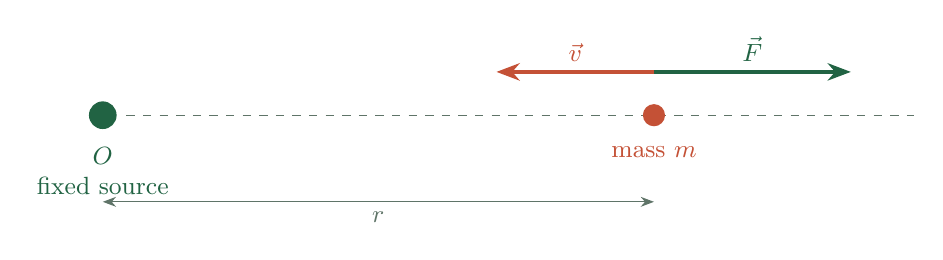
\begin{tikzpicture}[>=Stealth,font=\small]
  \fill[VectorAccent] (0,0) circle (5pt)
    node[below=8pt,align=center] {$O$\\fixed source};
  \draw[dashed,VectorMuted] (0.3,0)--(10.3,0);
  \fill[VectorCoral] (7,0) circle (4pt)
    node[below=8pt] {mass $m$};
  \draw[->,very thick,VectorCoral] (7,0.55)--(5,0.55)
    node[midway,above] {$\vec v$};
  \draw[->,very thick,VectorAccent] (7,0.55)--(9.5,0.55)
    node[midway,above] {$\vec F$};
  \draw[<->,VectorMuted] (0,-1.1)--node[below] {$r$}(7,-1.1);
\end{tikzpicture}
\end{center}

The approach is described by the following idealized readings, where
$\ell$ is a fixed length:
\begin{center}
\renewcommand{\arraystretch}{1.5}
\begin{tabular}{c|ccc}
Separation $r$ & $4\ell$ & $2\ell$ & $\ell$ \\
\hline
Squared speed $v^2$ & $\dfrac{63}{64}u^2$ & $\dfrac78u^2$ & $0$
\end{tabular}
\end{center}

\begin{enumerate}[label=\alph*)]
  \item Starting from Newton's second law and a dot product with velocity,
    find a relation between $F(r)$ and the slope of $v^2$ as a function of $r$.
  \item Suppose the deficit $u^2-v^2$ follows a power law in $r$.
    Use the readings to find a model for $v^2(r)$ and hence a closed
    expression for $F(r)$. Does doubling $r$ halve the force?
  \item The same particle now approaches the same source with incoming
    speed $2u$ very far away. Predict its closest separation, assuming
    your force law remains valid. Is this prediction within the range
    of separations in the table, or does it extend the model beyond them?
  \item At the turning point, the instantaneous rate of change of
    $v^2$ is zero. Must the force also be zero? Explain.
\end{enumerate}

\worklines{3}
\end{document}
